%!TEX root=/home/ska124/Dropbox/Thesis/thes-full.tex
%%%%%%%%%%%%%%%%%%%%%%%%%%%%%%%%%%%%%%%%%%%%%%%%%
%
%     Chapter 3   
%
%%%%%%%%%%%%%%%%%%%%%%%%%%%%%%%%%%%%%%%%%%%%%%%%%%%

\chapter{Amoeba Cache Architecture}
\label{chap:ac_architecture}

As described in Section \ref{sec:cache_memory_systems}, a conventional cache organises the data array into a 2 dimensional structure. A transparently addressed cache uses the same namespace (memory address space layout) as the main memory. The blocks which are stored in the sets are \textit{tagged} with the aligned start address of block present in the main memory. The \textit{tags} for the cache blocks currently present in the cache set are maintained in a separate array. When a search is being performed to find out whether a required physical address is present in the cache, the tag array is looked up to determine a cache hit or a cache miss. The organization of the cache set and tag array is shown in Figure \ref{fig:set_assoc_arch}. The effective address is the virtual address supplied by the CPU of the required datum. The component bits of the effective address is segmented into 3 parts which form the \textit{Virtual Page Number(VPN)}, set number and byte offset. The set number and byte offset are looked up in the tag array while the VPN is looked up in the \textit{Translation Lookaside Buffer(TLB)} to check that the current process has brought in the corresponding page and it is valid. The organisation described (and shown in Fig \ref{fig:set_assoc_arch}) is virtually indexed, physically tagged organisation where the lookup logic does not include the TLB translation in the critical path to enable faster searches. There are other organisations such as virtually indexed, virtually tagged and physically indexed, physically tagged which are uncommon due to inherent issues with their design. The tradeoff for a virtually indexed, physically tagged cache is that it can only grow in size with an increase in the associativity of each set, or an increase in the size of each cache block. The Intel Sandy Bridge architecture is known to use a virtually indexed, physically tagged cache organisation.



\begin{figure}[b]
  %% Pg 84 - Jacob
  \begin{center}
    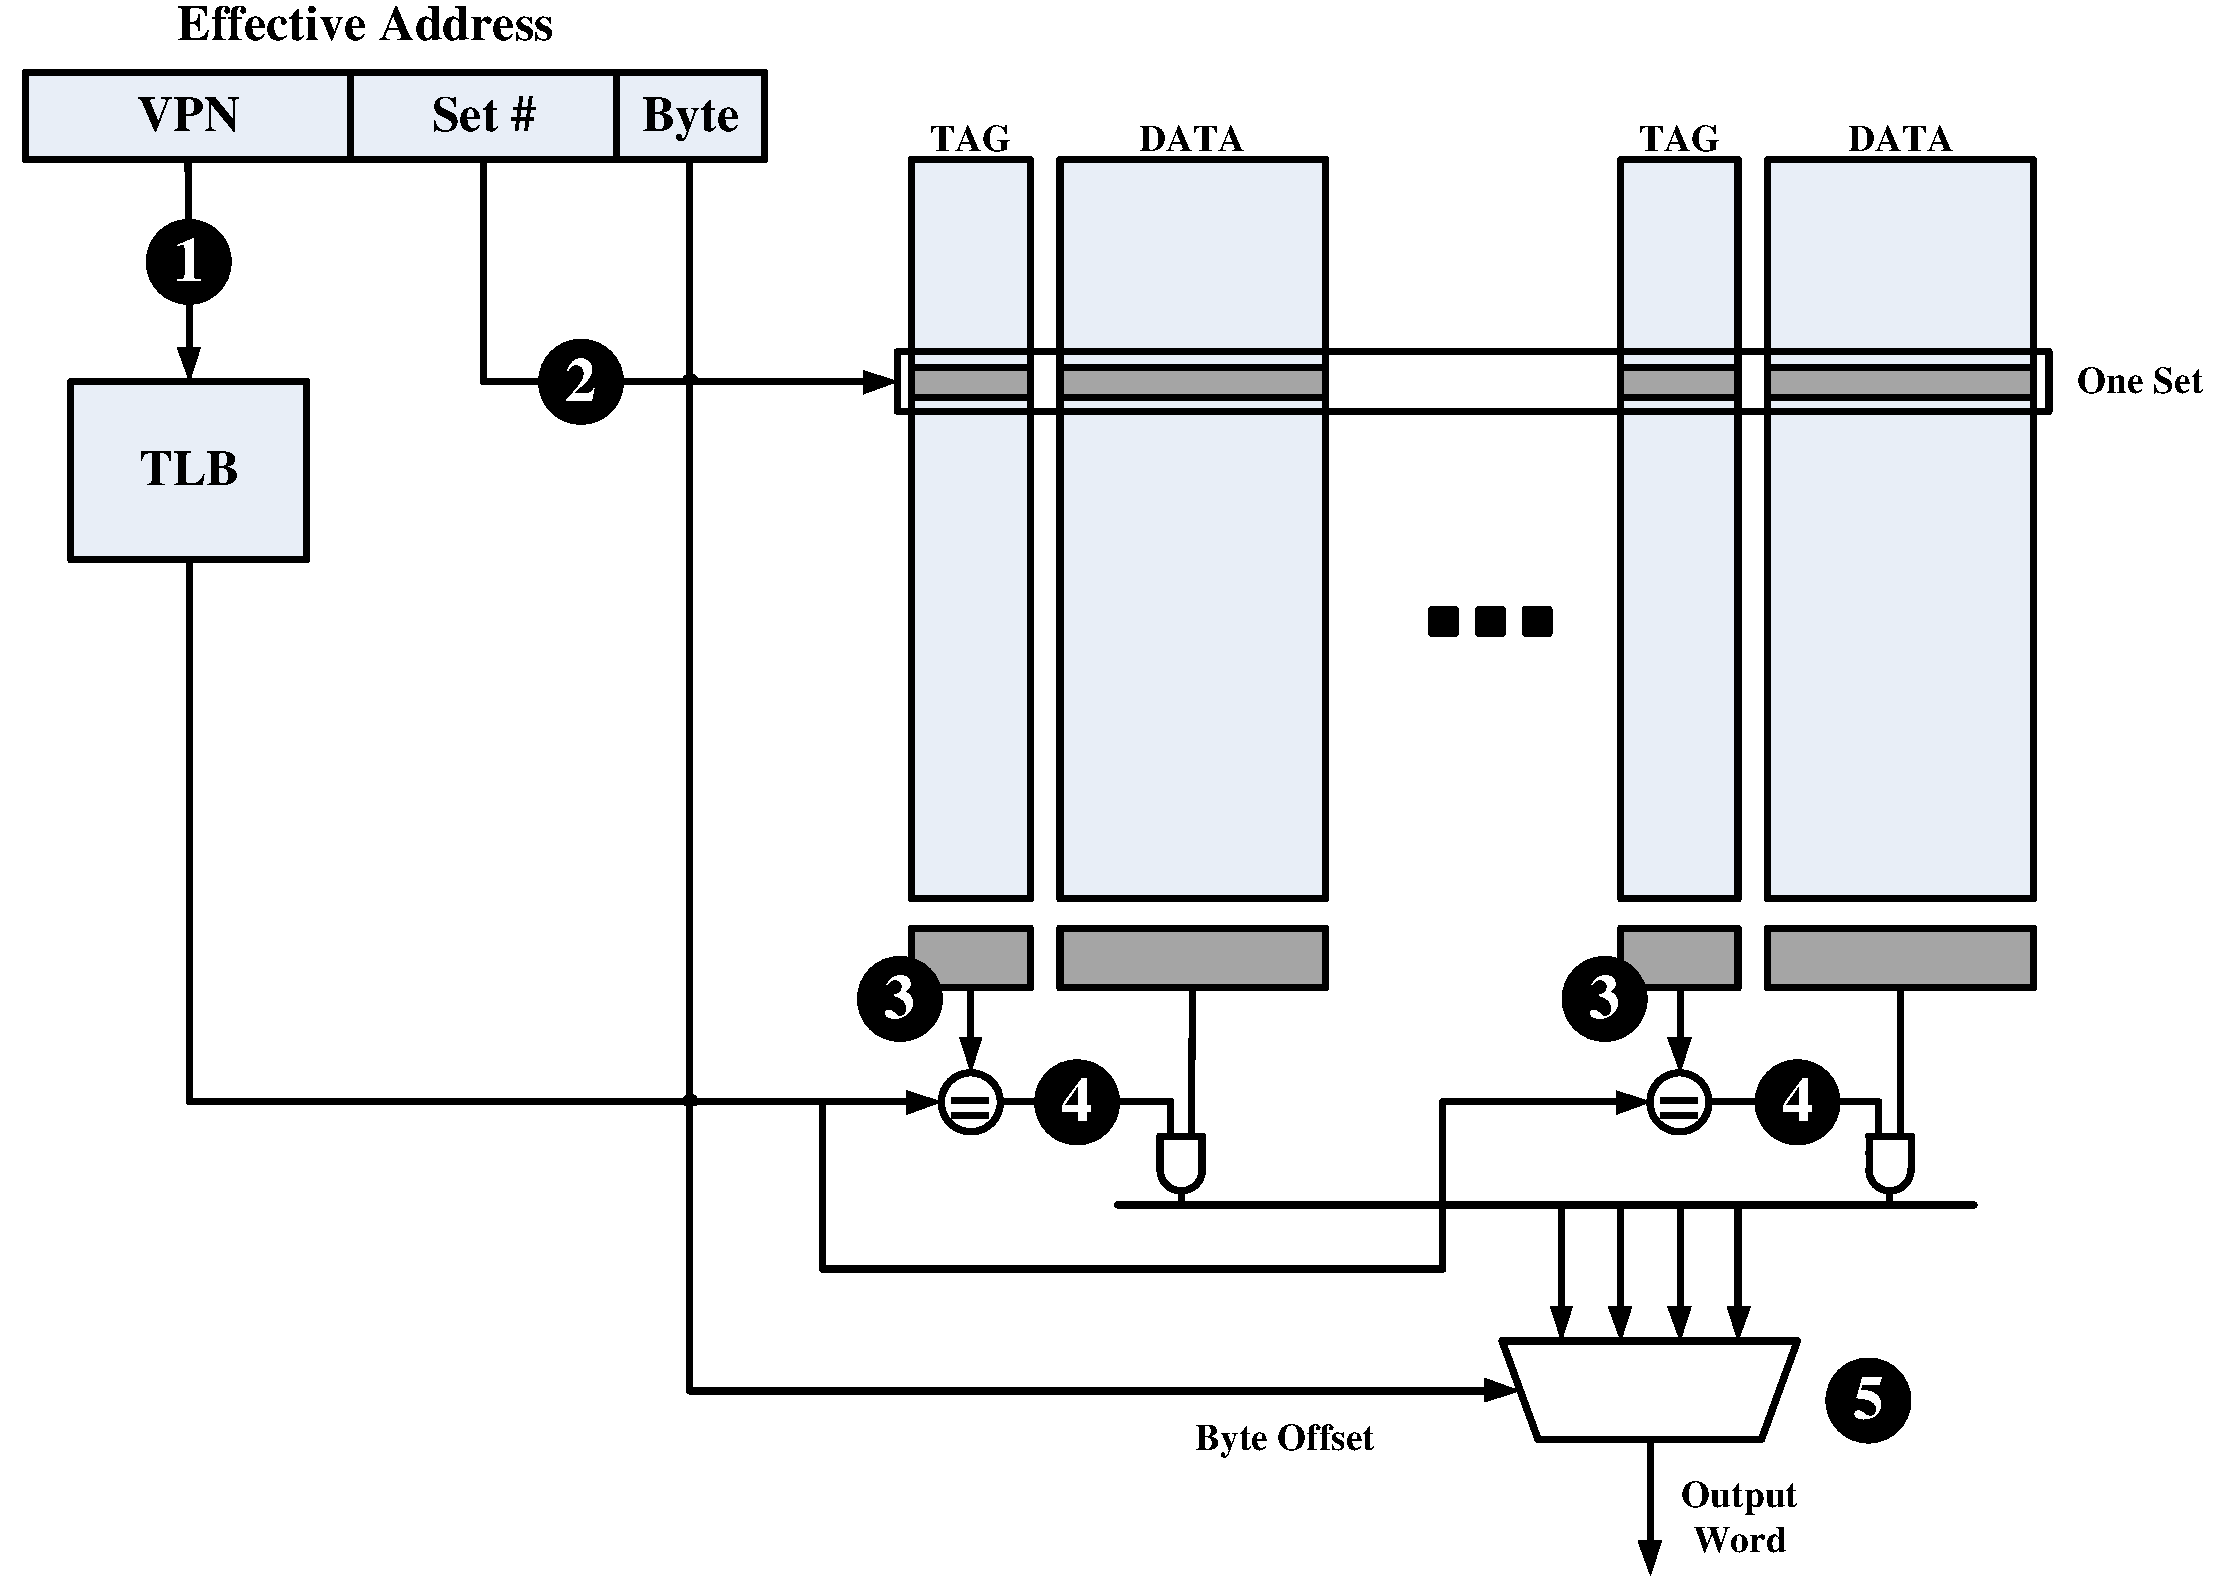
\includegraphics[width=\textwidth]{files/Figures/06-NWaySetAssocCache.pdf}
    \caption[Conventional N-Way Set-Associative Cache]{\textbf{Conventional N-Way Set-Associative Cache} \bigspot{1} The Virtual Page Number (VPN) is used to look up the entry in the Translation Lookaside Buffer (TLB) \bigspot{2} According to the number of sets in the cache, the following bits from the address are used to look up the corresponding set from the cache \bigspot{3} The tags read out from the set are compared with the translation from the TLB and tested for equality \bigspot{4} The corresponding cache block is forwarded to the output buffer for the tag which matches the TLB lookup \bigspot{5} Using the byte offset from the CPU, the mutiplexer selects the correponding critical word }
    \label{fig:set_assoc_arch}
  \end{center}
\end{figure}

\clearpage

In contrast to a conventional cache, the \AC\ architecture enables the memory hierarchy to fetch and allocate space for a range of words (i.e. a variable granularity cache block) based on the spatial locality of the application. For example, consider a 64K cache (256 sets) that allocates 256 bytes per set. These 256 bytes can adapt to support, for example, eight 32-bytes blocks, thirty-two 8-byte blocks, or four 32-byte blocks and sixteen 8-byte blocks, based on the set of contiguous words likely to be accessed. 
\\ \\
The key challenges to realising the \AC\ architecture are
\begin{enumerate}[noitemsep]
	\item To support a variable number of blocks per set
	\item To support a variable granularity for each block
	\item To support a variable number of tags, which correspond to the blocks in the set
\end{enumerate}

\begin{figure}[h]
  %% Pg 84 - Jacob
  \begin{center}
    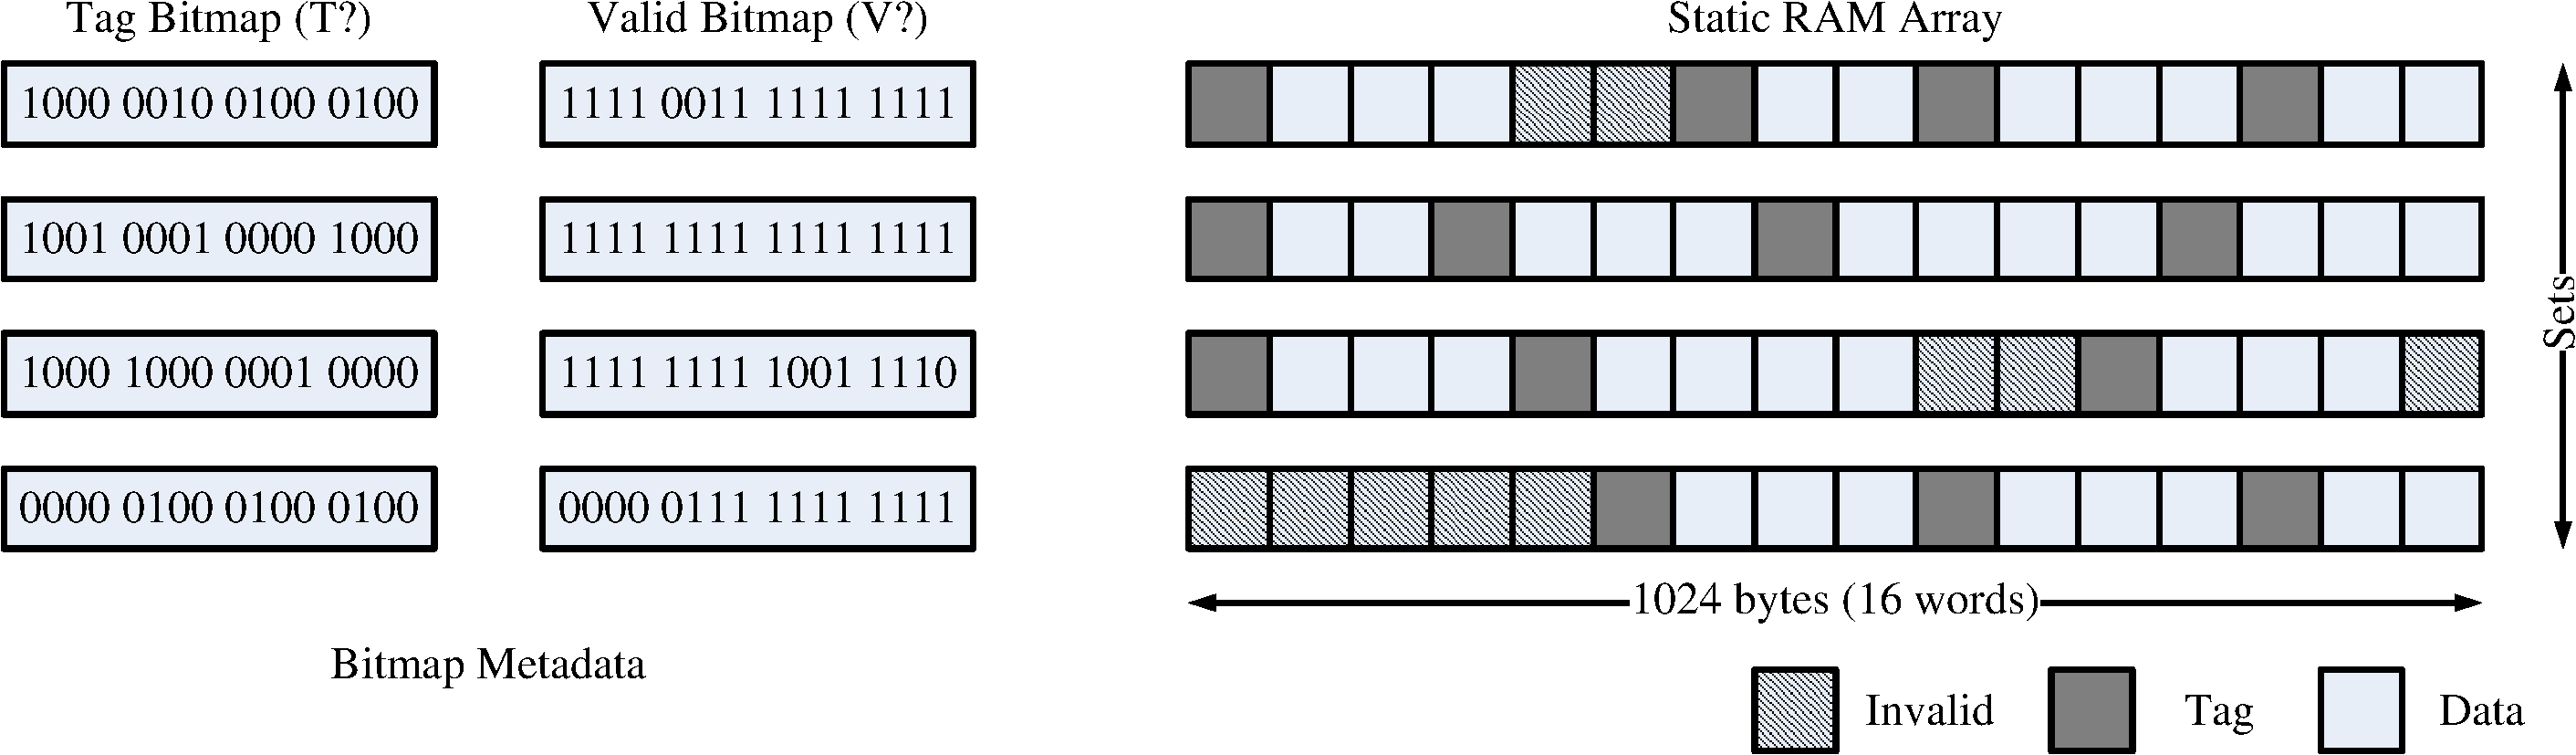
\includegraphics[width=\textwidth]{files/Figures/06-AmoebaCacheArch.pdf}
    \caption[Amoeba Cache Overview]{\textbf{Amoeba Cache Overview} The static RAM (SRAM) array where the tags and data are colocated is shown on the right. The \code{T? Bitmap} and the \code{V? Bitmap} for the \AC\ are shown on the left. Each block in the SRAM array represents 8 bytes (1 word). In this specific example, we show an \AC\ with 4 sets and 1024 bytes per set. The invalid, data and tag words (marked in the SRAM array) are tracked by setting the corresponding bits in the \code{T? and V? Bitmaps}. This information is maintained in order to simplify cache operations such as insertion and refill. }
    \label{fig:amoeba_cache_arch}
  \end{center}
\end{figure}

The \AC\ adopts a solution inspired by software data structures, where programs hold meta-data and actual data entries in the same address space. To achieve maximum flexibility, the \AC\ completely eliminates the tag array and collocates the tags with the actual data blocks (see Figure~\ref{fig:amoeba_cache_arch}). To distinguish which words are data words and which ones are tags within the set, we use a bitmap data structure (labeled \code{T? Bitmap} in Fig~\ref{fig:amoeba_cache_arch}). For each word in the set which is a tag, we set the corresponding bit in the \code{T? Bitmap}. We also decouple the conventional valid/invalid bits (typically associated with the tags) and organize them into a separate array (labeled \code{V? Bitmap} in Fig~\ref{fig:amoeba_cache_arch}) to simplify block replacement and insertion. \AC\ tags are composed of a \code{Region Tag} and a tuple which consists of the \code{Start} and \code{End} address of the variable granularity cache block. The data block immediately follows the tag word as shown in Fig~\ref{fig:amoeba_cache_arch}. The following sections provide more detail about the \AC\ architecture and how cache operations are performed.


\section{Amoeba Blocks and Set-Indexing}


\begin{figure}[h]
  %% Get images from http://en.wikipedia.org/wiki/CPU_cache#Associativity
  \subfloat[Memory Regions]{
    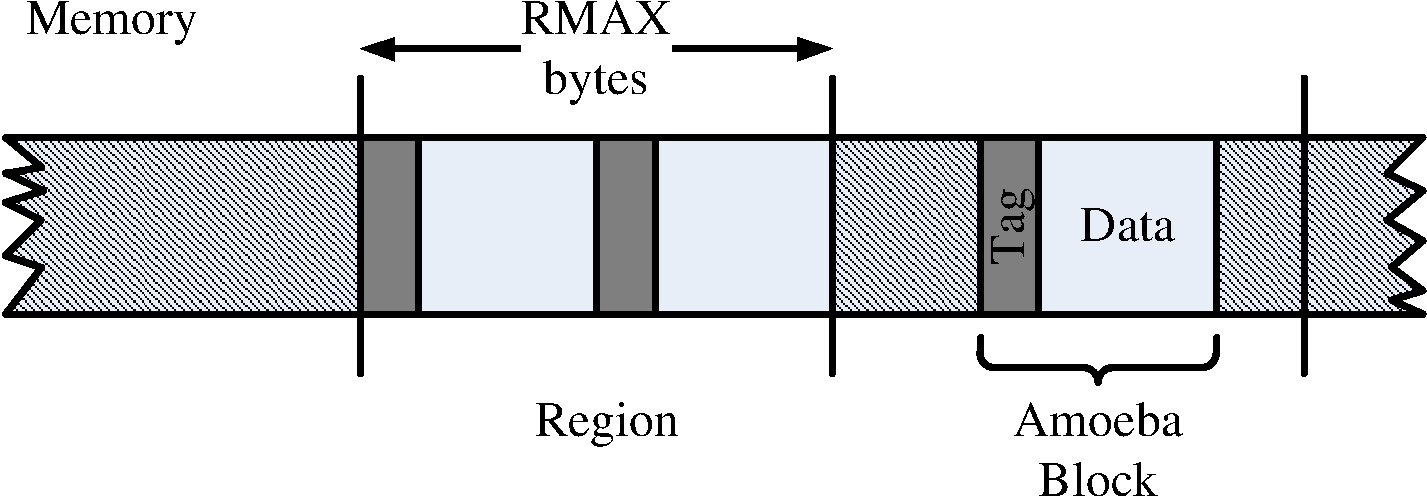
\includegraphics[width=0.5\textwidth]{files/Figures/06-MemoryRegions.pdf}
  }
  \subfloat[Addressing]{
     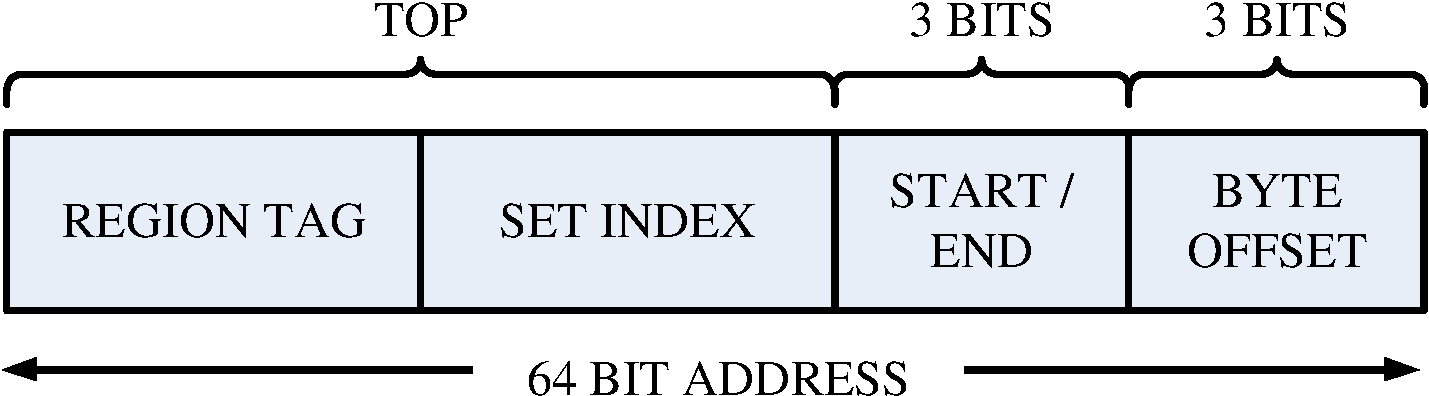
\includegraphics[width=0.5\textwidth]{files/Figures/06-Addressing.pdf}
  }
  \caption[Memory Regions]{ }
  \label{fig:mem_region_addr}
\end{figure}


The \AC\ data array holds a collection of varied granularity \AB{}s that do not overlap. Each \AB\ is a 4 tuple consisting of \code{\textless RegionTag, Start, End, Data-Block\textgreater} (Figure~\ref{fig:amoeba_cache_arch}). The first 3 components of the tuple are equivalent to a tag in a conventional cache. We allocate 8 bytes (1 word) for each tag. In order to simplify cache lookups for \AB{}s, we partition the address space into \code{Regions}. A \code{Region} is an aligned block of memory of size \code{RMAX} bytes. The boundaries of any \AB{} block (\code{Start} and \code{End}) are constrained to lie within the regions' boundaries. The minimum granularity of the data in an \AB\ is 1 word and the maximum is \code{RMAX} words. We can encode \code{Start} and \code{End} in $log_2(RMAX)$ bits. The set indexing function masks the lower $log_2(RMAX)$ bits to ensure that all \AB{}s (every memory word) from a region index to the same set. The Region Tag and Set-Index are identical for every word in the \AB{}. Retaining the notion of \textit{sets} enables fast lookups and helps elude challenges such as synonyms (same memory word mapping to different sets). When comparing against a conventional cache, we set \code{RMAX} to 8 words (64 bytes), ensuring that the set indexing function is identical to that in the conventional cache to allow for a fair evaluation.



% \subsection{Data Lookup}
% Figure~\ref{fig:Lookup} describes the steps of the lookup. \spot{1} The lower
% $log_2(RMAX)$ bits are masked from the address and the set index is derived
% from the remaining bits. \spot{2} In parallel with the data read out, the
% \code{T? bitmap} activates the words in the data array corresponding to the
% tags for comparison.  Note that given the minimum size of a \AB{} is two words
% (1 word for the tag metadata, 1 word for the data), adjacent words cannot be
% tags. We need $\frac{N_{words}}{2}$ 2-1 multiplexers that route one of the
% adjacent words to the comparator ($\in$ operator). The comparator generates
% the hit signal for the word selector. The $\in$ operator consists of two
% comparators: a) an aligned \code{Region tag} comparator, a conventional $==$
% (64 - $log_2N_{sets}$ - $log_2{RMAX}$ bits wide, e.g., 50 bits) that checks if
% the \AB{} belongs to the same region and b) a $ Start <= W < END $ range
% comparator ($log_2RMAX$ bits wide; e.g., 3 bits) that checks if the \AB\ holds
% the required word. Finally, in \spot{3}, the tag match activates and selects
% the appropriate word.



% \subsection{Amoeba Block Insertion}
% %
% On a miss for the desired word, a spatial granularity predictor is invoked
% (see Section~\ref{sec:predictors}), which specifies the range of the \AB{} to
% refill.
% %
% %\footnote{The spatial block range predictor is completely   independent
% %of the \AC\ design}. 
% %
% To determine a position in the set to slot the incoming
% block we can leverage the V? (Valid bits) bitmap. 
% The V? bitmap has 1 bit/word in the
% cache; a ``1'' bit indicates the word has been allocated (valid data or a
% tag). To find space for an incoming data block we perform a substring search
% on the V? bitmap of the cache set for contiguous 0s (empty words). For
% example, to insert an \AB{} of five words (four words for data and one word
% for tag), we perform a substring search for \textit{00000} in the V? bitmap /
% set (e.g., 32 bits wide for a 64K cache). If we cannot find the space, we keep
% triggering the replacement algorithm until we create the requisite contiguous
% space. Following this, the \AB\ tuple (Tag and Data block) is inserted, and
% the corresponding bits in the T? and V? array are set. The 0s substring search
% can be accomplished with a lookup table; 
% % estimated to require $\simeq$0.2ns using Cacti with a 32nm ITRS projection
% many current processors already include a substring
% instruction~\cite[PCMISTRI]{avxlatency}.

% \subsection{Replacement : Pseudo LRU}

% To reclaim the space from an \AB\, the tag bits T? (tag)
% and V? (valid) bits corresponding to the block are unset. The key issue is
% identifying the \AB\ to replace. Classical pseudo-LRU algorithms~\cite
% {Kedzierski-ipdps-2010,opensparct2,Kedzierski-ipdps-2010} keep the metadata
% for the replacement algorithm separate from the tags to reduce port
% contention.  \REVIEW{To be compatible with pseudo-LRU and other 
% algorithms such as DIP~\cite{qureshi-isca-2007} that work with a fixed 
% \# of ways, we can 
% logically partition a set in \AC\ into $N_{ways}$. For instance, if we
% partition a 32 word cache set into 4 logical ways, any access to
% an \AB\ tag found in words 0 ---7 of the set is treated as an access to
% logical way 0. Finding a replacement candidate involves identifying the
% selected replacement way and then picking (possibly randomly) a candidate \AB{}
% . More refined replacement algorithms that require per-tag metadata can
% harvest the space in the tag-word of the \AB\, which is 64 bits wide (for
%   alignment purposes) while physical addresses rarely extend beyond 48 bits.}



% \subsection{Partial Misses} \label{sec:partialmiss} 

% With variable granularity data blocks, a challenging although rare case (5
% in every 1K accesses) that occurs is a \textit{partial miss}. It is observed
% primarily when the spatial locality changes.  Figure~\ref{fig:partial-miss}
% shows an example. Initially, the set contains two blocks from a region R, one
% \AB\ caches words 1 --3 (Region:R, START:1 END:3) and the other holds words 5
% --6 (Region:R START:5 END:6). The CPU reads word 4, which
% misses, and the spatial predictor requests an \AB\ with range START:0 and
% END:7. The cache has \AB{}s that hold subparts of the incoming \AB{}, and some
% words (0, 4, and 7) need to be fetched.

% \AC\ removes the overlapping sub-blocks and allocates a new \AB{}. This is a
% multiple step process:\spot{1} On a miss, the cache identifies the overlapping
% sub-blocks in the cache using the tags read out during lookup. $\cap \neq
% NULL$ is true if $START_{new}$ < $END_{Tag}$ and $END_{new}$ > $START_{Tag}$
% ($New=$ incoming block and $Tag=$ \AB\ in set).  \spot{2} The data blocks that
% overlap with the miss range are evicted and moved one-at-a-time to the MSHR
% entry. \spot{3} Space is then allocated for the new block, i.e.,
% it is treated like a new insertion. \spot{4} A miss request is issued for the
% entire block (START:0 --- END:7) even if only some words (e.g., 0, 4, and 7)
% may be needed. This ensures request processing is simple and only a single
% refill request is sent.\spot{5} Finally, the incoming data block is patched
% into the MSHR; only the words not obtained from the L1 are copied (since the
% lower level could be stale).


% \begin{figure}[!h]
% \centering
% \includegraphics[width=0.37\textwidth]{figures/PartialMiss}
% \begin{minipage}[b]{0.5\textwidth} 
% { 
% \centering \spot{1}
%     Identify blocks overlapping with \code{New} block. \spot{2}
%     Evict overlapping blocks to MSHR. \spot{3} Allocate space
%     for new block (treat it like a new insertion). \spot{4} Issue
%     refill request to lower level for entire block. \spot{5} Patch
%     only newer words as lower-level data could be stale.  
% %(e.g., writeback cache)
% }
% \end{minipage}
% \caption{Partial Miss Handling. Upper: Identify relevant
%   sub-blocks. Useful for other cache controller events as well, e.g.,
%   recalls. Lower: Refill of words and insertion.}
% \label{fig:partial-miss}
% \end{figure}




% % \REVIEW{ Operations such as partial misses, replacements and invalidations,
% % which may require multiple steps, are modeled faithfully by the protocol. The
% % block is marked with state, $IV_C$ (a transient state) and separate protocol
% % events are triggered for each step. (see Section~\ref{sec:eval} for our
% % methodology). }

% %% Looking up the tag requires reading the data array.  This is extra
% %% energy cost. We may also need a lot of comparators.  Key question is
% %% how many comparators do you need. You don't want to provision too
% %% many. To minimize the \# of comparators needed in the common case we
% %% add filters to restrict the tag lookup when needed for a subset of the
% %% accesses.  We discuss two kinds of filters (1) Fast Tags : cache the
% %% tags themselves in a conventional tag array-like structure and with a
% %% pointer into the data array. A hit in this array ensures fast lookup.


% % \REVIEW{  The tags
% % collocated in the data array need to be touched during cache lookup and
% % insertion operations. Additionally they may need to be accessed during
% % coherence snoops at the L1, though our studies show that these operations are
% % infrequent (e.g., 1/100 cache operations in SpecJBB) and the directory and
% % inclusive LLC filter out most of the snoops. The proposed \textit{Fast Tags}
% % (Section~\ref{sec:extensions}) also act as a filter.}


% \section{Hardware Complexity}  \label{sec:physical}
%  We analyze the complexity of \AC\ along the following directions: we quantify the additions needed to the cache controller, we analyze the latency, area, and energy penalty, and finally, we study the challenges specifically introduced by large caches.

%  \subsection{Cache Controller} 

% \begin{figure}[!h]
% \centering
% \includegraphics[width=0.35\textwidth]{figures/L1Protocol}
% {
% \small
% \begin{tabular}{|@{~}c@{~}|@{~}p{2.75in}|} 
%       \multicolumn{2}{c}{Cache controller states}\\
%       \hline
%       State & Description \\
%       \hline
%       NP & \AB\ not present in the cache. \\
%       \hline
%       V & All words corresponding to \AB\ present and valid (read-only) \\
%       \hline
%       D & Valid and atleast one word in \AB\ is dirty (read-write) \\
%       \hline
%       {\bf IV\_B} & Partial miss being processed (blocking state) \\
%       \hline
%       {\bf IV\_Data} & Load miss; waiting for data from L2\\
%       \hline
%       ID\_Data & Store miss; waiting for data. Set dirty bit. \\
%       \hline
%       {\bf IV\_C} & Partial miss cleanup from cache completed (treat as full miss) \\
%       \hline
%       \multicolumn{2}{|c|}{\bf Amoeba-specific Cache Events}\\
%       \multicolumn{2}{|p{3in}|}{Partial miss: Process partial miss.} \\
%       \multicolumn{2}{|p{3in}|}{Local\_L1\_Evict: Remove overlapping \AB\ to MSHR.} \\
%       \multicolumn{2}{|p{3in}|}{Last\_L1\_Evict: Last \AB\ moved to MSHR. Convert to full miss and process load or store.} \\
%       \hline
%       \multicolumn{2}{p{3in}}{Bold and Broken-lines: \AC\ additions.} \\
%   \end{tabular}
%   }
% \caption{Amoeba Cache Controller (L1 level).}
%   \label{L1protocol}
% \end{figure}

% \REVIEW{The variable granularity \AB\ blocks need specific consideration in
% the cache controller. 
% %Note that the cache controller is needed to handle
% %interactions in a multi-level caches as well, not just coherence operations
% %(more details in \S~\ref{sec:coherence}). 
% %
% %
% We focus on the L1 controller here, and in particular, partial misses. 
% The cache controller manages operations at
% the aligned RMAX granularity. The controller  permits only one 
% in-flight cache operation per RMAX region.
% In-flight cache operations ensure no address overlap with stable 
% \AB{}s in order to eliminate complex race conditions.
% Figure~\ref{L1protocol} shows the L1 cache controller state machine. We add
% two states to the default protocol, \code{IV\_B} and \code{IV\_C}, 
% to handle partial misses. \code{IV\_B} is a blocking state that
% blocks other cache operations to RMAX region until all relevant \AB{}s to a
% partial miss are evicted (e.g., 0--3 and 5--7 blocks in Figure~\ref{fig:partial-miss}). 
% \code{IV\_C} indicates partial miss completion. This enables
% the controller to treat the access as a full miss and issue the refill request.
% The other stable states (I, V, D) and transient states (\code{IV\_Data} and
% \code{ID\_Data}) are present in a conventional protocol as well. \code
% {Partial-miss} triggers the clean-up
% operations (\code{1} and \code{2} in Figure~\ref{fig:partial-miss}).
% \code{Local\_L1\_Evict} is a looping event that keeps retriggering
% for each \AB\ involved in the partial miss; \code{Last\_L1\_Evict} is
% triggered when the last \AB\ involved in the partial miss is evicted to the MSHR. 
% A key difference between the L1 and lower-level protocols is that the Load/Store
% event in the lower-level protocol may need to access data from multiple \AB{}s. 
% In such cases,
% similar to the partial-miss event, we read out each block independently before
% supplying the data (more details in \S~\ref{sec:multicache}).
%  }


% \subsection{Area, Latency, and Energy Overhead}
% The extra metadata required by \AC\ are the T? (1 tag bit per word) and V? (1
% valid bit per word) bitmaps. Table~\ref{table:overheads} shows the quantitative
% overhead compared to the data storage. Both the T? and V?  bitmap
% arrays are directly proportional to the size of the cache and require a
% constant storage overhead (3\% in total). The T? bitmap is read in parallel
% with the data array and does not affect the critical path; T? adds 2\%---3.5\%
% (depending on cache size) to the overall cache access energy. 
% V? is referred only on misses when inserting a new block.

% \begin{table}[!htb]
% {
% \vspace{-10pt}
% \centering
% \caption{\AC\ Hardware Complexity.}
% \label{table:overheads}
% {
% \small 
% \begin{tabular}{|@{~}c@{~}|@{~}c@{~}|@{~}c@{~}|@{~}c@{~}|}
% \hline
% \multicolumn{4}{|c|}{Cache configuration}\\
% \hline
%              & 64K (256by/set) & 1MB (512by/set) & 4MB (1024by/set) \\
% \hline
% \multicolumn{4}{|l|}{Data RAM parameters} \\   
% \hline
% Delay        & 0.36ns & 2ns & 2.5 ns \\
% Energy       & 100pJ & 230pJ  & 280pJ \\
% \hline 
% \multicolumn{4}{|c|}{\AC\ components (CACTI model)} \\   
% \hline
% T?/V? map & 1KB &  16KB & 64KB \\
% Latency      & 0.019ns (5\%) & 0.12ns (6\%) & 0.2ns (6\%) \\   
% Energy       & 2pJ (2\%) & 8pJ (3.4\%) & 10pJ (3.5\%)  \\ 
% LRU  & $\frac{1}{8}$KB & 2KB & 8KB \\
% \hline
% \multicolumn{4}{|c|}{Lookup Overhead (VHDL model)} \\
% \hline
% Area    & 0.7\% & \multicolumn{2}{c|}{0.1\%} \\  
% \hline
% Latency & 0.02ns & 0.035ns & 0.04ns \\
% \hline
% \end{tabular}
% }

% {
%   \% indicates overhead compared to data array of cache. 64K cache operates in \textit{Fast mode}; 1MB and
%   4MB operate in \textit{Normal mode}. We use 32nm ITRS HP transistors for
%   64K and 32nm ITRS LOP transistors for 1MB and 4MB.
% }
% }
% \end{table}

% We synthesized\footnote{We do not have access to an industry-grade 32nm library, 
% so we synthesized at a higher 180nm node size and scaled the results to 32 nm 
% (latency and energy scaled proportional to Vdd (taken from~\cite{cpudb}) 
% and $Vdd^2$ respectively).}
%  the cache lookup logic using Synopsys and quantify the area,
% latency, and energy penalty. \AC\ is compatible with  \textit{Fast} and
% \textit{Normal} cache access modes~\cite[-access-mode config]{muralimanohar-
% micro-2007}, both of which read the entire set from the data array in parallel
% with the way selection to  achieve lower latency.  \textit{Fast} mode
% transfers the entire set to the edge of the H-tree, while  \textit{Normal}
% mode, only transmits the selected way over the H-tree. For synthesis, we used
% the Synopsys design compiler (Vision Z-2007.03-SP5).



% Figure~\ref{fig:Lookup} shows \AC\'s lookup hardware on the critical path; 
% we compare it
% against a fixed-granularity cache's lookup logic (mainly the comparators). The
% area overhead of the \AC\ includes registering an entire line that has been
% read out, the tag operation logic, and the word selector. The components on the
% critical path once the data is read out are the 2-way multiplexers, the $\in$
% comparators, and priority encoder that selects the word; the T?  bitmap is
% accessed in parallel and off the critical path. \AC\ is made feasible under
% today's wire-limited technology where the cache latency and energy is
% dominated by the bit/word lines, decoder, and H-tree~\cite{muralimanohar- micro-2007}.  \AC{}'s comparators, which operate on
% the entire cache set, are 6$\times$ the area of a fixed cache's comparators. 
% Note that the data array occupies 99\% of the overall cache area. The critical
% path is dominated by the wide word selector since the comparators all
% operate in parallel. The lookup logic adds 60\% to the conventional cache's
% comparator time. The overall critical path is dominated by the data array
% access and \AC{}'s lookup circuit adds 0.02ns to the access latency and
% $\simeq$ 1pJ to the energy of a 64K cache, and 0.035ns to the latency and
% $\simeq$2pJ to the energy of a 1MB cache. Finally, \AC\ amortizes the energy
% penalty of the peripheral components (H-tree, Wordline, and decoder) over a
% single RAM. 


% \REVIEW{\AC{}'s overhead needs careful consideration when implemented at the L1
% cache level. We have two options for handling the latency overhead a) if the L1
% cache is the critical stage in the pipeline, we can throttle the CPU clock by
% the latency overhead to ensure that the additional logic fits within the
% pipeline stage. This ensures that the number of pipeline stages for a memory
% access does not change with respect to a conventional cache, although all
% instructions bear the overhead of the reduced CPU clock. b) we can add an
% extra pipeline stage to the L1 hit path, adding a 1 cycle overhead to all
% memory accesses but ensuring no change in CPU frequency. We quantify the
% performance impact of both approaches in Section~\ref{sec:eval}.}


% \subsection{Tag-only Operations}  Conventional caches support tag-only
% operations to reduce data port contention. While the \AC\ merges tags and
% data, like many commercial processors it decouples the replacement metadata
% and valid bits from the tags, accessing the tags only on cache lookup. Lookups
% can be either CPU side or network side (coherence invalidation and
% Wback/Forwarding). CPU-side lookups and writebacks ($\simeq$ 95\% of cache
% operations) both need data and hence \AC\ in the common case does not
% introduce extra overhead. \AC\ does read out the entire data array unlike
% serial-mode caches (we discuss this issue in the next section). Invalidation
% checks and snoops can be more energy expensive with \AC{} compared to a
% conventional cache. Fortunately, coherence snoops are not common in many
% applications (e.g., 1/100 cache operations in SpecJBB) as a coherence
% directory and an inclusive LLC filter them out.


% \subsection{Tradeoff with Large Caches} \label{sec:extensions}
% \begin{figure}[!ht] \centering
% \begin{minipage}[c]{0.4\textwidth} {
% \includegraphics[width=\textwidth]{plots/predictors/Serial_vs_Normal.pdf}
% }
% \end{minipage}
% \begin{minipage}[c]{0.4\textwidth}
% {
% Baseline: Serial. $\leq1$ Normal is better.  32nm, ITRS  LOP.
% } 
% \end{minipage}  
% \caption{Serial vs Normal mode cache.}
% \label{fig:serial_parallel} 
% \end{figure}

% Large caches with many words per set ($\equiv$ highly associative conventional
% cache) need careful consideration.  \REVIEW{ Typically, highly associative
% caches tend to serialize tag and data access with only the relevant cache
% block read out on a hit and no data access on a miss. We first analyze the the
% tradeoff between reading the entire set (normal mode), which is compatible with
% \AC\, and only the relevant block (serial mode). } We vary the cache size from
% 2M---8M and associativity from 4(256B/set) --- 32 (2048B/set).  Under current
% technology constraints (Figure~\ref{fig:serial_parallel}), only at very high
% associativity does serial mode demonstrate a notable energy benefit. Large
% caches are dominated by H-tree energy consumption and reading out the entire
% set at each sub-bank imposes an energy penalty when bitlines and wordlines
% dominate (2KB+ \# of words/set).

% \begin{table}[!h]
% \begin{center}
% \vspace{-10pt}
% \caption{\% of direct accesses with fast tags}
% \label{fig:tagcount}
% {
% \small
% \begin{tabular}{|@{~}p{0.6in}@{~}|@{~}c@{~}|@{~}c@{~}|@{~}c@{~}|@{~}c@{~}|@{~}c@{~}|@{~}c@{~}|}
% \hline
% % \multicolumn{7}{|@{~}c@{~}|}{Cache Size}\\
%   &  \multicolumn{2}{@{~}c@{~}|} {64K(256by/set)} &  \multicolumn{2}{@{~}c@{~}|} {1MB(512by/set)} & \multicolumn{2}{@{~}c@{~}|} {2MB(1024 by/set)} \\
% \hline
% \# Tags/set &2 &  4 & 4 & 8 & 8 & 16 \\

% Overhead &  1KB & 2KB  & 2KB & 16KB  & 16KB & 32KB  \\  
% \hline
% {Benchmarks} & & & & & & \\

% Low      & 30\% & 45\% & 42\% & 64\% & 55\% & 74\%\\
% Moderate & 24\% & 62\% & 46\% & 70\% & 63\% & 85\%\\
% High     & 35\% & 79\% & 67\% & 95\% & 75\% & 96\%\\
% \hline
% \end{tabular}
% }
% \vspace{-10pt}
% \end{center}
% \end{table}


% \REVIEW{\AC\ can be tuned to minimize the hardware overhead for large caches.
% With many words/set the cache utilization improves due to longer block
% lifetimes making it feasible to support \AB{}s with a larger minimum
% granularity ($>$ 1 word). If we increase minimum granularity to two or four
% words, only every third or fifth word could be a tag, meaning the \# of
% comparators and multiplexers reduce to $\frac{N_{words/set}}{3}$ or
% $\frac{N_{words/set}}{5}$. When the minimum granularity is equal to max
% granularity (RMAX), we obtain a fixed granularity cache with
% $N_{words/set}/RMAX$ ways. Cache organizations that collocate all the tags
% together at the head of the data array enable tag-only operations and serial
% \AB\ accesses that need to activate only a portion of the data array. However, the set may need to be compacted at each insertion. Recently, Loh and Hill~\cite{loh- hill-micro-2011} explored such an organization for
% supporting tags in multi-gigabyte caches.}


% Finally, the use of \textit{Fast Tags} help reduce the tag lookups in the
% data array. Fast tags use a separate traditional tag array-like structure to
% cache the tags of the recently-used blocks and provide a pointer directly to
% the \AB{}. The \# of \textit{Fast Tags} needed per set is proportional to the
% \# of blocks in each set, which varies with the spatial locality in the
% application and the \# of bytes per set (more details in
% Section~\ref{sec:efficiency}). We studied 3 different cache configurations
% (64K 256B/set, 1M 512B/set, and 2M 1024B/set) while varying the number of 
% fast tags per set (see Table~\ref{fig:tagcount}). 
% With 8 tags/set (16KB
% overhead), we can filter 64---95\% of the accesses in a 1MB cache and 55---
% 75\% of the accesses in a 2MB cache.
